\chapter{Open Shortest Path First}
\label{chap:ospf}

Open Shortest Path First (OSPF) is by far the most popular and important
routing protocol in use today---so important, I'm devoting this entire
chapter to it! Sticking with the same approach we've adhered to
throughout this book, we'll begin with the basics by completely
familiarizing you with key OSPF terminology. Once we've covered that
thoroughly, I'll guide you through OSPF's internal operation and then
move on to tell you all about OSPF's many advantages over RIP.

This chapter is going to be more than chock full of vitally important
information and it's also going to be really exciting because together,
we'll explore some seriously critical factors and issues innate to
implementing OSPF! I'll walk you through exactly how to implement
single-area OSPF in a variety of networking environments and then
demonstrate some great techniques you'll need to verify that everything
is configured correctly and running smoothly.



\section{Open Shortest Path First (OSPF) Basics}

\emph{Open Shortest Path First} is an open standard routing protocol
that's been implemented by a wide variety of network vendors, including
Cisco. And it's that open standard characteristic that's the key to
OSPF's flexibility and popularity.

Most people opt for OSPF, which works by using the Dijkstra algorithm to
initially construct a shortest path tree and follows that by populating
the routing table with the resulting best paths. EIGRP's convergence
time may be blindingly fast, but OSPF isn't that far behind, and its
quick convergence is another reason it's a favorite. Another two great
advantages OSPF offers are that it supports multiple, equal-cost routes
to the same destination and, like EIGRP, it also supports both IP and
IPv6 routed protocols.

Here's a list that summarizes some of OSPF's best features:

\begin{enumerate}
\tightlist
\item
  Allows for the creation of areas and autonomous systems
\item
  Minimizes routing update traffic
\item
  Is highly flexible, versatile, and scalable
\item
  Supports VLSM/CIDR
\item
  \protect\hypertarget{c18.xhtmlux5cux23Page_747}{}{}Offers an unlimited
  hop count
\item
  Is open standard and supports multi-vendor deployment
\end{enumerate}

Because OSPF is the first link-state routing protocol that most people
run into, it's a good idea to size it up against more traditional
distance-vector protocols like RIPv2 and RIPv1.
\protect\hyperlink{c18.xhtmlux5cux23table18-1}{Table 18.1} presents a
nice comparison of all three of these common protocols.

{\protect\hyperlink{c18.xhtmlux5cux23tableanchor18-1}{\textbf{TABLE~18.1}}
OSPF and RIP comparison}

\begin{longtable}[]{@{}llll@{}}
\toprule
Characteristic & OSPF & RIPv2 & RIPv1\tabularnewline
\midrule
\endhead
Type of protocol & Link state & Distance vector & Distance
vector\tabularnewline
Classless support & Yes & Yes & No\tabularnewline
VLSM support & Yes & Yes & No\tabularnewline
Auto-summarization & No & Yes & Yes\tabularnewline
Manual summarization & Yes & Yes & No\tabularnewline
Noncontiguous support & Yes & Yes & No\tabularnewline
Route propagation & Multicast on change & Periodic multicast & Periodic
broadcast\tabularnewline
Path metric & Bandwidth & Hops & Hops\tabularnewline
Hop count limit & None & 15 & 15\tabularnewline
Convergence & Fast & Slow & Slow\tabularnewline
Peer authentication & Yes & Yes & No\tabularnewline
Hierarchical network requirement & Yes (using areas) & No (flat only) &
No (flat only)\tabularnewline
Updates & Event triggered & Periodic & Periodic\tabularnewline
Route computation & Dijkstra & Bellman-Ford &
Bellman-Ford\tabularnewline
\bottomrule
\end{longtable}

I want you know that OSPF has many features beyond the few I've listed
in \protect\hyperlink{c18.xhtmlux5cux23table18-1}{Table 18.1}, and all
of them combine to produce a fast, scalable, robust protocol that's also
flexible enough to be actively deployed in a vast array of production
networks!

One of OSPF's most useful traits is that its design is intended to be
hierarchical in use, meaning that it allows us to subdivide the larger
internetwork into smaller internetworks
\protect\hypertarget{c18.xhtmlux5cux23Page_748}{}{}called areas. It's a
really powerful feature that I recommend using, and I promise to show
you how to do that later in the chapter.

Here are three of the biggest reasons to implement OSPF in a way that
makes full use of its intentional, hierarchical design:

\begin{enumerate}
\tightlist
\item
  To decrease routing overhead
\item
  To speed up convergence
\item
  To confine network instability to single areas of the network
\end{enumerate}

Because free lunches are invariably hard to come by, all this wonderful
functionality predictably comes at a price and doesn't exactly make
configuring OSPF any easier. But no worries---we'll crush it!

Let's start by checking out
\protect\hyperlink{c18.xhtmlux5cux23figure18-1}{Figure 18.1}, which
shows a very typical, yet simple OSPF design. I really want to point out
the fact that some routers connect to the backbone---called area 0---the
backbone area. OSPF absolutely must have an area 0, and all other areas
should connect to it except for those connected via virtual links, which
are beyond the scope of this book. A router that connects other areas to
the backbone area within an AS is called an \emph{area border router
(ABR)}, and even these must have at least one of their interfaces
connected to area 0.

\begin{figure}
\centering
%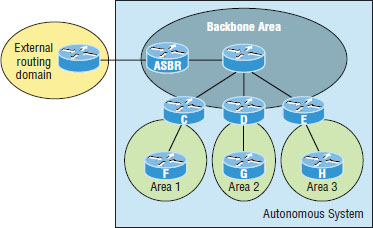
\includegraphics{images/c18f001.jpg}
\caption{{\protect\hyperlink{c18.xhtmlux5cux23figureanchor18-1}{\textbf{FIGURE
18.1}} OSPF design example. An OSPF hierarchical design minimizes
routing table entries and keeps the impact of any topology changes
contained within a specific area.}}
\end{figure}

OSPF runs great inside an autonomous system, but it can also connect
multiple autonomous systems together. The router that connects these ASs
is called an \emph{autonomous system boundary router (ASBR)}. Ideally,
your aim is to create other areas of networks to help keep route updates
to a minimum, especially in larger networks. Doing this also keeps
problems from propagating throughout the network, effectively isolating
them to a single area.

But let's pause here to cover some key OSPF terms that are really
essential for you to nail down before we move on any further.

\subsubsection[OSPF
Terminology]{\texorpdfstring{\protect\hypertarget{c18.xhtmlux5cux23c18-sec-2}{}{}\protect\hypertarget{c18.xhtmlux5cux23Page_749}{}{}OSPF
Terminology}{OSPF Terminology}}

Imagine being given a map and compass with no prior concept of east,
west, north or south---not even what rivers, mountains, lakes, or
deserts are. I'm guessing that without any ability to orient yourself in
a basic way, your cool, new tools wouldn't help you get anywhere but
completely lost, right? This is exactly why we're going to begin
exploring OSPF by getting you solidly acquainted with a fairly long list
of terms before setting out from base camp into the great unknown! Here
are those vital terms to commit to memory now:

\textbf{Link} A \emph{link} is a network or router interface assigned to
any given network. When an interface is added to the OSPF process, it's
considered to be a link. This link, or interface, will have up or down
state information associated with it as well as one or more IP
addresses.

\textbf{Router ID} The \emph{router ID (RID)} is an IP address used to
identify the router. Cisco chooses the router ID by using the highest IP
address of all configured loopback interfaces. If no loopback interfaces
are configured with addresses, OSPF will choose the highest IP address
out of all active physical interfaces. To OSPF, this is basically the
``name'' of each router.

\textbf{Neighbor} \emph{Neighbors} are two or more routers that have an
interface on a common network, such as two routers connected on a
point-to-point serial link. OSPF neighbors must have a number of common
configuration options to be able to successfully establish a neighbor
relationship, and all of these options must be configured exactly the
same way:

\begin{enumerate}
\tightlist
\item
  Area ID
\item
  Stub area flag
\item
  Authentication password (if using one)
\item
  Hello and Dead intervals
\end{enumerate}

\textbf{Adjacency} An \emph{adjacency} is a relationship between two
OSPF routers that permits the direct exchange of route updates. Unlike
EIGRP, which directly shares routes with all of its neighbors, OSPF is
really picky about sharing routing information and will directly share
routes only with neighbors that have also established adjacencies. And
not all neighbors will become adjacent---this depends upon both the type
of network and the configuration of the routers. In multi-access
networks, routers form adjacencies with designated and backup designated
routers. In point-to-point and point-to-multipoint networks, routers
form adjacencies with the router on the opposite side of the connection.

\textbf{Designated router} A \emph{designated router (DR)} is elected
whenever OSPF routers are connected to the same broadcast network to
minimize the number of adjacencies formed and to publicize received
routing information to and from the remaining routers on the broadcast
network or link. Elections are won based upon a router's priority level,
with the one having the highest priority becoming the winner. If there's
a tie, the router ID will be used to break it. All routers on the shared
network will establish adjacencies with the DR and the BDR, which
ensures that all routers' topology tables are synchronized.

\protect\hypertarget{c18.xhtmlux5cux23Page_750}{}{}\textbf{Backup
designated router} A \emph{backup designated router (BDR)} is a hot
standby for the DR on broadcast, or multi-access, links. The BDR
receives all routing updates from OSPF adjacent routers but does not
disperse LSA updates.

\textbf{Hello protocol} The OSPF Hello protocol provides dynamic
neighbor discovery and maintains neighbor relationships. Hello packets
and Link State Advertisements (LSAs) build and maintain the topological
database. Hello packets are addressed to multicast address 224.0.0.5.

\textbf{Neighborship database} The \emph{neighborship database} is a
list of all OSPF routers for which Hello packets have been seen. A
variety of details, including the router ID and state, are maintained on
each router in the neighborship database.

\textbf{Topological database} The \emph{topological database} contains
information from all of the Link State Advertisement packets that have
been received for an area. The router uses the information from the
topology database as input into the Dijkstra algorithm that computes the
shortest path to every network.

\begin{center}\rule{0.5\linewidth}{0.5pt}\end{center}

%\includegraphics{images/note.png}
LSA packets are used to update and
maintain the topological database.

\begin{center}\rule{0.5\linewidth}{0.5pt}\end{center}

\textbf{Link State Advertisement} A \emph{Link State Advertisement
(LSA)} is an OSPF data packet containing link-state and routing
information that's shared among OSPF routers. An OSPF router will
exchange LSA packets only with routers to which it has established
adjacencies.

\textbf{OSPF areas} An \emph{OSPF area} is a grouping of contiguous
networks and routers. All routers in the same area share a common area
ID. Because a router can be a member of more than one area at a time,
the area ID is associated with specific interfaces on the router. This
would allow some interfaces to belong to area 1 while the remaining
interfaces can belong to area 0. All of the routers within the same area
have the same topology table. When configuring OSPF with multiple areas,
you've got to remember that there must be an area 0 and that this is
typically considered the backbone area. Areas also play a role in
establishing a hierarchical network organization---something that really
enhances the scalability of OSPF!

\textbf{Broadcast (multi-access)} \emph{Broadcast (multi-access)
networks} such as Ethernet allow multiple devices to connect to or
access the same network, enabling a \emph{broadcast} ability in which a
single packet is delivered to all nodes on the network. In OSPF, a DR
and BDR must be elected for each broadcast multi-access network.

\textbf{Nonbroadcast multi-access} \emph{Nonbroadcast multi-access
(NBMA)} networks are networks such as Frame Relay, X.25, and
Asynchronous Transfer Mode (ATM). These types of networks allow for
multi-access without broadcast ability like Ethernet. NBMA networks
require special OSPF configuration to function properly.

\protect\hypertarget{c18.xhtmlux5cux23Page_751}{}{}\textbf{Point-to-point}
\emph{Point-to-point} refers to a type of network topology made up of a
direct connection between two routers that provides a single
communication path. The point-to-point connection can be physical---for
example, a serial cable that directly connects two routers---or logical,
where two routers thousands of miles apart are connected by a circuit in
a Frame Relay network. Either way, point-to-point configurations
eliminate the need for DRs or BDRs.

\textbf{Point-to-multipoint} \emph{Point-to-multipoint} refers to a type
of network topology made up of a series of connections between a single
interface on one router and multiple destination routers. All interfaces
on all routers share the point-to-multipoint connection and belong to
the same network. Point-to-multipoint networks can be further classified
according to whether they support broadcasts or not. This is important
because it defines the kind of OSPF configurations you can deploy.

All of these terms play a critical role when you're trying to understand
how OSPF actually works, so again, make sure you're familiar with each
of them. Having these terms down will enable you to confidently place
them in their proper context as we progress on our journey through the
rest of this chapter!

\subsubsection[OSPF
Operation]{\texorpdfstring{\protect\hypertarget{c18.xhtmlux5cux23c18-sec-3}{}{}OSPF
Operation}{OSPF Operation}}

Fully equipped with your newly acquired knowledge of the terms and
technologies we just covered, it's now time to delve into how OSPF
discovers, propagates, and ultimately chooses routes. Once you know how
OSPF achieves these tasks, you'll understand how OSPF operates
internally really well.

OSPF operation is basically divided into these three categories:

\begin{enumerate}
\tightlist
\item
  Neighbor and adjacency initialization
\item
  LSA flooding
\item
  SPF tree calculation
\end{enumerate}

The beginning neighbor/adjacency formation stage is a very big part of
OSPF operation. When OSPF is initialized on a router, the router
allocates memory for it, as well as for the maintenance of both neighbor
and topology tables. Once the router determines which interfaces have
been configured for OSPF, it will then check to see if they're active
and begin sending Hello packets as shown in
\protect\hyperlink{c18.xhtmlux5cux23figure18-2}{Figure 18.2}.

\begin{figure}
\centering
%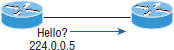
\includegraphics{images/c18f002.jpg}
\caption{{\protect\hyperlink{c18.xhtmlux5cux23figureanchor18-2}{\textbf{FIGURE
18.2}} The Hello protocol}}
\end{figure}

The Hello protocol is used to discover neighbors, establish adjacencies,
and maintain relationships with other OSPF routers. Hello packets are
periodically sent out of each enabled OSPF interface and in environments
that support multicast.

\protect\hypertarget{c18.xhtmlux5cux23Page_752}{}{}The address used for
this is 224.0.0.5, and the frequency with which Hello packets are sent
out depends upon the network type and topology. Broadcast and
point-to-point networks send Hellos every 10 seconds, whereas
non-broadcast and point-to-multipoint networks send them every 30
seconds.

\paragraph{LSA Flooding}

\emph{LSA flooding} is the method OSPF uses to share routing
information. Via Link State Updates (LSU's) packets, LSA information
containing link-state data is shared with all OSPF routers within an
area. The network topology is created from the LSA updates, and flooding
is used so that all OSPF routers have the same topology map to make SPF
calculations with.

Efficient flooding is achieved through the use of a reserved multicast
address: 224.0.0.5 (AllSPFRouters). LSA updates, which indicate that
something in the topology has changed, are handled a bit differently.
The network type determines the multicast address used for sending
updates. \protect\hyperlink{c18.xhtmlux5cux23table18-2}{Table 18.2}
contains the multicast addresses associated with LSA flooding.
Point-to-multipoint networks use the adjacent router's unicast IP
address.

{\protect\hyperlink{c18.xhtmlux5cux23tableanchor18-2}{\textbf{TABLE~18.2}}
LSA update multicast addresses}

\begin{longtable}[]{@{}lll@{}}
\toprule
Network Type & Multicast Address & Description\tabularnewline
\midrule
\endhead
Point-to-point & 224.0.0.5 & AllSPFRouters\tabularnewline
Broadcast & 224.0.0.6 & AllDRouters\tabularnewline
Point-to-multipoint & NA & NA\tabularnewline
\bottomrule
\end{longtable}

Once the LSA updates have been flooded throughout the network, each
recipient must acknowledge that the flooded update has been received.
It's also important for recipients to validate the LSA update.

\paragraph{SPF Tree Calculation}

Within an area, each router calculates the best/shortest path to every
network in that same area. This calculation is based upon the
information collected in the topology database and an algorithm called
shortest path first (SPF). Picture each router in an area constructing a
tree---much like a family tree---where the router is the root and all
other networks are arranged along the branches and leaves. This is the
shortest-path tree used by the router to insert OSPF routes into the
routing table.

It's important to understand that this tree contains only networks that
exist in the same area as the router itself does. If a router has
interfaces in multiple areas, then separate trees will be constructed
for each area. One of the key criteria considered during the route
selection process of the SPF algorithm is the metric or cost of each
potential path to a network. But this SPF calculation doesn't apply to
routes from other areas.

\subparagraph[OSPF
Metrics]{\texorpdfstring{\protect\hypertarget{c18.xhtmlux5cux23c18-sec-4}{}{}\protect\hypertarget{c18.xhtmlux5cux23Page_753}{}{}OSPF
Metrics}{OSPF Metrics}}

OSPF uses a metric referred to as \emph{cost}. A cost is associated with
every outgoing interface included in an SPF tree. The cost of the entire
path is the sum of the costs of the outgoing interfaces along the path.
Because cost is an arbitrary value as defined in RFC 2338, Cisco had to
implement its own method of calculating the cost for each OSPF-enabled
interface. Cisco uses a simple equation of
10\textsuperscript{8}/\emph{bandwidth}, where \emph{bandwidth} is the
configured bandwidth for the interface. Using this rule, a 100 Mbps Fast
Ethernet interface would have a default OSPF cost of 1 and a 1,000 Mbps
Ethernet interface would have a cost of 1.

Important to note is that this value can be overridden with the
\texttt{ip\ ospf\ cost} command. The cost is manipulated by changing the
value to a number within the range of 1 to 65,535. Because the cost is
assigned to each link, the value must be changed on the specific
interface you want to change the cost on.

\begin{center}\rule{0.5\linewidth}{0.5pt}\end{center}

%\includegraphics{images/note.png}
Cisco bases link cost on bandwidth.
Other vendors may use other metrics to calculate a given link's cost.
When connecting links between routers from different vendors, you'll
probably have to adjust the cost to match another vendor's router
because both routers must assign the same cost to the link for OSPF to
work properly.

\begin{center}\rule{0.5\linewidth}{0.5pt}\end{center}



\section{Configuring OSPF}

Configuring basic OSPF isn't as simple as configuring RIP and EIGRP, and
it can get really complex once the many options that are allowed within
OSPF are factored in. But that's okay because you really only need to
focus on basic, single-area OSPF configuration at this point. Coming up,
I'll show you how to configure single-area OSPF.

The two factors that are foundational to OSPF configuration are enabling
OSPF and configuring OSPF areas.

\subsubsection[Enabling
OSPF]{\texorpdfstring{\protect\hypertarget{c18.xhtmlux5cux23c18-sec-6}{}{}Enabling
OSPF}{Enabling OSPF}}

The easiest and also least scalable way to configure OSPF is to just use
a single area. Doing this requires a minimum of two commands.

The first command used to activate the OSPF routing process is as
follows:

\begin{verbatim}
Router(config)#router ospf ?
<1-65535> Process ID
\end{verbatim}

A value in the range from 1 to 65,535 identifies the OSPF process ID.
It's a unique number on this router that groups a series of OSPF
configuration commands under a specific running process. Different OSPF
routers don't have to use the same process ID to communicate. It's a
purely local value that doesn't mean a lot, but you still need to
remember that it cannot start at 0; it has to start at a minimum of 1.

\protect\hypertarget{c18.xhtmlux5cux23Page_754}{}{}You can have more
than one OSPF process running simultaneously on the same router if you
want, but this isn't the same as running multi-area OSPF. The second
process will maintain an entirely separate copy of its topology table
and manage its communications independently of the first one and you use
it when you want OSPF to connect multiple ASs together. Also, because
the Cisco exam objectives only cover single-area OSPF with each router
running a single OSPF process, that's what we'll focus on in this book.

\begin{center}\rule{0.5\linewidth}{0.5pt}\end{center}

%\includegraphics{images/note.png}
The OSPF process ID is needed to
identify a unique instance of an OSPF database and is locally
significant.

\begin{center}\rule{0.5\linewidth}{0.5pt}\end{center}

\subsubsection[Configuring OSPF
Areas]{\texorpdfstring{\protect\hypertarget{c18.xhtmlux5cux23c18-sec-7}{}{}Configuring
OSPF Areas}{Configuring OSPF Areas}}

After identifying the OSPF process, you need to identify the interfaces
that you want to activate OSPF communications on as well as the area in
which each resides. This will also configure the networks you're going
to advertise to others.

Here's an example of a basic OSPF configuration for you, showing our
second minimum command needed, the \texttt{network} command:

\begin{verbatim}
Router#config t
Router(config)#router ospf 1
Router(config-router)#network 10.0.0.0 0.255.255.255 area ?
  <0-4294967295>  OSPF area ID as a decimal value
  A.B.C.D         OSPF area ID in IP address format
Router(config-router)#network 10.0.0.0 0.255.255.255 area 0
\end{verbatim}

\begin{center}\rule{0.5\linewidth}{0.5pt}\end{center}

%\includegraphics{images/note.png}
The areas can be any number from 0 to
4.2 billion. Don't get these numbers confused with the process ID, which
ranges from 1 to 65,535.

\begin{center}\rule{0.5\linewidth}{0.5pt}\end{center}

Remember, the OSPF process ID number is irrelevant. It can be the same
on every router on the network, or it can be different---doesn't matter.
It's locally significant and just enables the OSPF routing on the
router.

The arguments of the \texttt{network} command are the network number
(10.0.0.0) and the wildcard mask (0.255.255.255). The combination of
these two numbers identifies the interfaces that OSPF will operate on
and will also be included in its OSPF LSA advertisements. Based on my
sample configuration, OSPF will use this command to find any interface
on the router configured in the 10.0.0.0 network and will place any
interface it finds into area 0.
\protect\hypertarget{c18.xhtmlux5cux23Page_755}{}{}Notice that you can
create about 4.2 billion areas! In reality, a router wouldn't let you
create that many, but you can certainly name them using the numbers up
to 4.2 billion. You can also label an area using an IP address format.

Let me stop here a minute to give you a quick explanation of wildcards:
A 0 octet in the wildcard mask indicates that the corresponding octet in
the network must match exactly. On the other hand, a 255 indicates that
you don't care what the corresponding octet is in the network number. A
network and wildcard mask combination of 1.1.1.1 0.0.0.0 would match an
interface configured exactly with 1.1.1.1 only, and nothing else. This
is really useful if you want to activate OSPF on a specific interface in
a very clear and simple way. If you insist on matching a range of
networks, the network and wildcard mask combination of 1.1.0.0
0.0.255.255 would match any interface in the range of 1.1.0.0 to
1.1.255.255. Because of this, it's simpler and safer to stick to using
wildcard masks of 0.0.0.0 and identify each OSPF interface individually.
Once configured, they'll function exactly the same---one way really
isn't better than the other.

The final argument is the area number. It indicates the area to which
the interfaces identified in the network and wildcard mask portion
belong. Remember that OSPF routers will become neighbors only if their
interfaces share a network that's configured to belong to the same area
number. The format of the area number is either a decimal value from the
range 0 to 4,294,967,295 or a value represented in standard
dotted-decimal notation. For example, area 0.0.0.0 is a legitimate area
and is identical to area 0.

\paragraph{Wildcard Example}

Before getting down to configuring our network, let's take a quick peek
at a more complex OSPF network configuration to find out what our OSPF
network statements would be if we were using subnets and wildcards.

In this scenario, you have a router with these four subnets connected to
four different interfaces:

\begin{enumerate}
\tightlist
\item
  192.168.10.64/28
\item
  192.168.10.80/28
\item
  192.168.10.96/28
\item
  192.168.10.8/30
\end{enumerate}

All interfaces need to be in area 0, so it seems to me the easiest
configuration would look like this:

\begin{verbatim}
Test#config t
Test(config)#router ospf 1
Test(config-router)#network 192.168.10.0 0.0.0.255 area 0
\end{verbatim}

I'll admit that the preceding example is actually pretty simple, but
easy isn't always best---especially when dealing with OSPF! So even
though this is an easy-button way to configure OSPF, it doesn't make
good use of its capabilities and what fun is that? Worse
\protect\hypertarget{c18.xhtmlux5cux23Page_756}{}{}yet, the objectives
aren't very likely to present something this simple for you! So let's
create a separate network statement for each interface using the subnet
numbers and wildcards. Doing that would look something like this:

\begin{verbatim}
Test#config t
Test(config)#router ospf 1
Test(config-router)#network 192.168.10.64 0.0.0.15 area 0
Test(config-router)#network 192.168.10.80 0.0.0.15 area 0
Test(config-router)#network 192.168.10.96 0.0.0.15 area 0
Test(config-router)#network 192.168.10.8 0.0.0.3 area 0
\end{verbatim}

Wow, now that's a different looking config! Truthfully, OSPF would work
exactly the same way as it would with the easy configuration I showed
you first---but unlike the easy configuration, this one covers the
objectives!

And although this looks a bit complicated, trust me, it really isn't.
All you need for clarity is to fully understand your block sizes! Just
remember that when configuring wildcards, they're always one less than
the block size. A /28 is a block size of 16, so we would add our network
statement using the subnet number and then add a wildcard of 15 in the
interesting octet. For the /30, which is a block size of 4, we would go
with a wildcard of 3. Once you practice this a few times, it gets really
easy. And do practice because we'll deal with them again when we get to
access lists later on!

Let's use \protect\hyperlink{c18.xhtmlux5cux23figure18-3}{Figure 18.3}
as an example and configure that network with OSPF using wildcards to
make sure you have a solid grip on this. The figure shows a three-router
network with the IP addresses of each interface.

\begin{figure}
\centering
%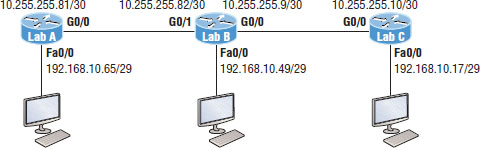
\includegraphics{images/c18f003.jpg}
\caption{{\protect\hyperlink{c18.xhtmlux5cux23figureanchor18-3}{\textbf{FIGURE
18.3}} Sample OSPF wildcard configuration}}
\end{figure}

The very first thing you need to be able to do is to look at each
interface and determine the subnet that the addresses are in. Hold on, I
know what you're thinking: ``Why don't I just use the exact IP addresses
of the interface with the 0.0.0.0 wildcard?'' Well, you can, but we're
paying attention to Cisco exam objectives here, not just what's easiest,
remember?

\protect\hypertarget{c18.xhtmlux5cux23Page_757}{}{}The IP addresses for
each interface are shown in the figure. The Lab\_A router has two
directly connected subnets: 192.168.10.64/29 and 10.255.255.80/30.
Here's the OSPF configuration using wildcards:

\begin{verbatim}
Lab_A#config t
Lab_A(config)#router ospf 1
Lab_A(config-router)#network 192.168.10.64 0.0.0.7 area 0
Lab_A(config-router)#network 10.255.255.80 0.0.0.3 area 0
\end{verbatim}

The Lab\_A router is using a /29, or 255.255.255.248, mask on the Fa0/0
interface. This isa block size of 8, which is a wildcard of 7. The G0/0
interface is a mask of 255.255.255.252---block size of 4, with a
wildcard of 3. Notice that I typed in the network number, not the
interface number. You can't configure OSPF this way if you can't look at
the IP address and slash notation and then figure out the subnet, mask,
and wildcard, can you? So don't take your exam until you can do this.

Here are other two configurations to help you practice:

\begin{verbatim}
Lab_B#config t
Lab_B(config)#router ospf 1
Lab_B(config-router)#network 192.168.10.48 0.0.0.7 area 0
Lab_B(config-router)#network 10.255.255.80 0.0.0.3 area 0
Lab_B(config-router)#network 10.255.255.8 0.0.0.3 area 0
 
Lab_C#config t
Lab_C(config)#router ospf 1
Lab_C(config-router)#network 192.168.10.16 0.0.0.7 area 0
Lab_C(config-router)#network 10.255.255.8 0.0.0.3 area 0
\end{verbatim}

As I mentioned with the Lab\_A configuration, you've got to be able to
determine the subnet, mask, and wildcard just by looking at the IP
address and mask of an interface. If you can't do that, you won't be
able to configure OSPF using wildcards as I just demonstrated. So go
over this until you're really comfortable with it!

\subsubsection[Configuring Our Network with
OSPF]{\texorpdfstring{\protect\hypertarget{c18.xhtmlux5cux23c18-sec-8}{}{}Configuring
Our Network with OSPF}{Configuring Our Network with OSPF}}

Now we get to have some fun! Let's configure our internetwork with OSPF
using just area 0. OSPF has an administrative distance of 110, but let's
remove RIP while we're at it because I don't want you to get in the
habit of having RIP running on your network.

There's a bunch of different ways to configure OSPF, and as I said, the
simplest and easiest is to use the wildcard mask 0.0.0.0. But I want to
demonstrate that we can configure each router differently with OSPF and
still come up with the exact same result. This is one reason why OSPF is
more fun and challenging than other routing protocols---it gives us all
a lot more ways to screw things up, which automatically provides
\protect\hypertarget{c18.xhtmlux5cux23Page_758}{}{}a troubleshooting
opportunity! We'll use our network as shown in
\protect\hyperlink{c18.xhtmlux5cux23figure18-4}{Figure 18.4} to
configure OSPF, and by the way, notice I added a new router!

\begin{figure}
\centering
%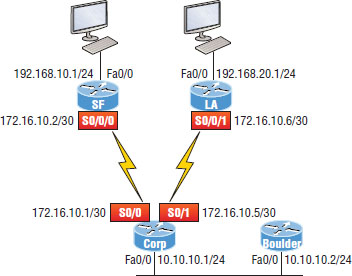
\includegraphics{images/c18f004.jpg}
\caption{{\protect\hyperlink{c18.xhtmlux5cux23figureanchor18-4}{\textbf{FIGURE
18.4}} Our new network layout}}
\end{figure}

\paragraph{Corp}

Here's the Corp router's configuration:

\begin{verbatim}
Corp#sh ip int brief
Interface        IP-Address      OK? Method Status                Protocol
FastEthernet0/0  10.10.10.1      YES manual up                    up
Serial0/0        172.16.10.1     YES manual up                    up
FastEthernet0/1  unassigned      YES unset  administratively down down
Serial0/1        172.16.10.5     YES manual up                    up
Corp#config t
Corp(config)#no router rip
Corp(config)#router ospf 132
Corp(config-router)#network 10.10.10.1 0.0.0.0 area 0
Corp(config-router)#network 172.16.10.1 0.0.0.0 area 0
Corp(config-router)#network 172.16.10.5 0.0.0.0 area 0
\end{verbatim}

Alright---it looks like we have a few things to talk about here. First,
I removed RIP and then added OSPF. Why did I use OSPF 132? It really
doesn't matter---the number is irrelevant. I guess it just felt good to
use 132. But notice that I started with the
\texttt{show\ ip\ int\ brief} command, just like when I was configuring
RIP. I did this because it's always
\protect\hypertarget{c18.xhtmlux5cux23Page_759}{}{}important to verify
exactly what you are directly connected to. Doing this really helps
prevent typos!

The network commands are pretty straightforward. I typed in the IP
address of each interface and used the wildcard mask of 0.0.0.0, which
means that the IP address must precisely match each octet. This is
actually one of those times where easier is better, so just do this:

\begin{verbatim}
Corp(config)#router ospf 132
Corp(config-router)#network 172.16.10.0 0.0.0.255 area 0
\end{verbatim}

Nice---there's only one line instead of two for the 172.16.10.0 network!
I really want you to understand that OSPF will work the same here no
matter which way you configure the network statement. Now, let's move on
to SF. To simplify things, we're going to use our same sample
configuration.

\paragraph{SF}

The SF router has two directly connected networks. I'll use the IP
addresses on each interface to configure this router.

\begin{verbatim}
SF#sh ip int brief
Interface    IP-Address      OK? Method Status                Protocol
FastEthernet0/0  192.168.10.1    YES manual up                    up
FastEthernet0/1  unassigned      YES unset  administratively down down
Serial0/0/0      172.16.10.2     YES manual up                    up
Serial0/0/1      unassigned      YES unset  administratively down down
SF#config t
SF(config)#no router rip
SF(config)#router ospf 300
SF(config-router)#network 192.168.10.1 0.0.0.0 area 0
SF(config-router)#network 172.16.10.2 0.0.0.0 area 0
*Apr 30 00:25:43.810: %OSPF-5-ADJCHG: Process 300, Nbr 172.16.10.5 on Serial0/0/0 from LOADING to FULL, Loading Done
\end{verbatim}

Here, all I did was to first disable RIP, turn on OSPF routing process
300, and then I added my two directly connected networks. Now let's move
on to LA!

\paragraph{LA}

We're going to give some attention to the LA router that's directly
connected to two networks:

\begin{verbatim}
LA#sh ip int brief
Interface    IP-Address      OK? Method Status                Protocol
FastEthernet0/0 192.168.20.1    YES manual up                    up
FastEthernet0/1 unassigned      YES unset  administratively down down
Serial0/0/0     unassigned      YES unset  administratively down down
Serial0/0/1     172.16.10.6     YES manual up                    up
LA#config t
LA(config)#router ospf 100
LA(config-router)#network 192.168.20.0 0.0.0.255 area 0
LA(config-router)#network 172.16.0.0 0.0.255.255 area 0
*Apr 30 00:56:37.090: %OSPF-5-ADJCHG: Process 100, Nbr 172.16.10.5 on Serial0/0/1 from LOADING to FULL, Loading Done
\end{verbatim}

Remember that when you're configuring dynamic routing, using the
\texttt{show\ ip\ int\ brief} command first will make it all so much
easier!

And don't forget, I can use any process ID I want, as long as it's a
value from 1 to 65,535, because it doesn't matter if all routers use the
same process ID. Also, notice that I used different wildcards in this
example. Doing this works really well too.

Okay, I want you to think about something for a second before we move
onto more advanced OSPF topics: What if the Fa0/1 interface of the LA
router was connected to a link that we didn't need OSPF running on, as
shown in \protect\hyperlink{c18.xhtmlux5cux23figure18-5}{Figure 18.5}?

\begin{figure}
\centering
%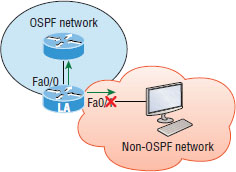
\includegraphics{images/c18f005.jpg}
\caption{{\protect\hyperlink{c18.xhtmlux5cux23figureanchor18-5}{\textbf{FIGURE
18.5}} Adding a non-OSPF network to the LA router}}
\end{figure}

You've seen this before because I demonstrated this already back in the
RIP section. We can use the same command that we did under that routing
process here as well! Take a look:

\begin{verbatim}
LA(config)#router ospf 100
LA(config-router)#passive-interface fastEthernet 0/1
\end{verbatim}

Even though this is pretty simple, you've really got to be careful
before you configure this command on your router! I added this command
as an example on interface Fa0/1, which happens to be an interface we're
not using in this network because I want OSPF to work on my other
router's interfaces.

\protect\hypertarget{c18.xhtmlux5cux23Page_761}{}{}Now it's time to
configure our Corp router to advertise a default route to the SF and LA
routers because doing so will make our lives a lot easier. Instead of
having to configure all our routers with a default route, we'll only
configure one router and then advertise that this router is the one that
holds the default route---elegant!

In \protect\hyperlink{c18.xhtmlux5cux23figure18-4}{Figure 18.4}, keep in
mind that, for now, the corporate router is connected to the Internet
off of Fa0/0. We'll create a default route toward this imaginary
Internet and then tell the other routers that this is the route they'll
use to get to the Internet. Here is the configuration:

\begin{verbatim}
Corp#config t
Corp(config)#ip route 0.0.0.0 0.0.0.0 Fa0/0
Corp(config)#router ospf 1
Corp(config-router)#default-information originate
\end{verbatim}

Now, let's check and see if our other routers have received this default
route from the Corp router:

\begin{verbatim}
SF#show ip route
[output cut]
E1 - OSPF external type 1, E2 - OSPF external type 2
[output cut]
O*E2 0.0.0.0/0 [110/1] via 172.16.10.1, 00:01:54, Serial0/0/0
SF#
\end{verbatim}

Sure enough---the last line in the SF router shows that it received the
advertisement from the Corp router regarding the fact that the corporate
router is the one holding the default route out of the AS.

But hold on a second! I need to configure our new router into my lab to
create the example network we'll use from here on. Here's the
configuration of the new router that I connected to the same network
that the Corp router is connected to via the Fa0/0 interface:

\begin{verbatim}
Router#config t
Router(config)#hostname Boulder
Boulder(config)#int f0/0
Boulder(config-if)#ip address 10.10.10.2 255.255.255.0
Boulder(config-if)#no shut
*Apr  6 18:01:38.007: %LINEPROTO-5-UPDOWN: Line protocol on Interface FastEthernet0/0, changed state to up
Boulder(config-if)#router ospf 2
Boulder(config-router)#network 10.0.0.0 0.255.255.255 area 0
*Apr  6 18:03:27.267: %OSPF-5-ADJCHG: Process 2, Nbr 223.255.255.254 on FastEthernet0/0 from LOADING to FULL, Loading Done
\end{verbatim}

This is all good, but I need to make sure that you don't follow my
example to a tee because here, I just quickly brought a router up
without setting my passwords first. I can
\protect\hypertarget{c18.xhtmlux5cux23Page_762}{}{}get away with this
only because I am in a nonproduction network, so don't do this in the
real world where security is key!

Anyway, now that I have my new router nicely connected with a basic
configuration, we're going to move on to cover loopback interfaces, how
to set the router ID (RID) used with OSPF, and finally, how to verify
OSPF.



\section{OSPF and Loopback Interfaces}

It's really vital to configure loopback interfaces when using OSPF. In
fact, Cisco suggests using them whenever you configure OSPF on a router
for stability purposes.

\emph{Loopback interfaces} are logical interfaces, which means they're
virtual, software-only interfaces, not actual, physical router
interfaces. A big reason we use loopback interfaces with OSPF
configurations is because they ensure that an interface is always active
and available for OSPF processes.

Loopback interfaces also come in very handy for diagnostic purposes as
well as for OSPF configuration. Understand that if you don't configure a
loopback interface on a router, the highest active IP address on a
router will become that router's RID during bootup!
\protect\hyperlink{c18.xhtmlux5cux23figure18-6}{Figure 18.6} illustrates
how routers know each other by their router ID.

\begin{figure}
\centering
%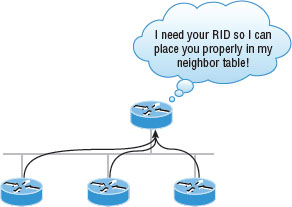
\includegraphics{images/c18f006.jpg}
\caption{{\protect\hyperlink{c18.xhtmlux5cux23figureanchor18-6}{\textbf{FIGURE
18.6}} OSPF router ID (RID)}}
\end{figure}

The RID is not only used to advertise routes, it's also used to elect
the designated router (DR) and the backup designated router (BDR). These
designated routers create adjacencies when a new router comes up and
exchanges LSAs to build topological databases.

\begin{center}\rule{0.5\linewidth}{0.5pt}\end{center}

%\includegraphics{images/note.png}
By default, OSPF uses the highest IP
address on any active interface at the moment OSPF starts up to
determine the RID of the router. But this behavior can be overridden via
a logical interface. Remember---the highest IP address of any logical
interface will always become a router's RID!

\begin{center}\rule{0.5\linewidth}{0.5pt}\end{center}

\protect\hypertarget{c18.xhtmlux5cux23Page_763}{}{}Now it's time to show
you how to configure these logical loopback interfaces and how to verify
them, as well as verify RIDs.

\subsubsection[Configuring Loopback
Interfaces]{\texorpdfstring{\protect\hypertarget{c18.xhtmlux5cux23c18-sec-10}{}{}Configuring
Loopback Interfaces}{Configuring Loopback Interfaces}}

Configuring loopback interfaces rocks mostly because it's the easiest
part of OSPF configuration, and we all need a break about now---right?
So hang on---we're in the home stretch!

First, let's see what the RID is on the Corp router with the
\texttt{show\ ip\ ospf} command:

\begin{verbatim}
Corp#sh ip ospf
 Routing Process "ospf 1" with ID 172.16.10.5
[output cut]
\end{verbatim}

Okay, we can see that the RID is 172.16.10.5---the Serial0/1 interface
of the router. So let's configure a loopback interface using a
completely different IP addressing scheme:

\begin{verbatim}
Corp(config)#int loopback 0
*Mar 22 01:23:14.206: %LINEPROTO-5-UPDOWN: Line protocol on Interface
   Loopback0, changed state to up
Corp(config-if)#ip address 172.31.1.1 255.255.255.255
\end{verbatim}

The IP scheme really doesn't matter here, but each one being in a
separate subnet does! By using the /32 mask, we can use any IP address
we want as long as the addresses are never the same on any two routers.

Let's configure the other routers now:

\begin{verbatim}
SF#config t
SF(config)#int loopback 0
*Mar 22 01:25:11.206: %LINEPROTO-5-UPDOWN: Line protocol on Interface
   Loopback0, changed state to up
SF(config-if)#ip address 172.31.1.2 255.255.255.255
\end{verbatim}

Here's the configuration of the loopback interface on LA:

\begin{verbatim}
LA#config t
LA(config)#int loopback 0
*Mar 22 02:21:59.686: %LINEPROTO-5-UPDOWN: Line protocol on Interface
   Loopback0, changed state to up
LA(config-if)#ip address 172.31.1.3 255.255.255.255
\end{verbatim}

I'm pretty sure you're wondering what the IP address mask of
255.255.255.255 (/32) means and why we don't just use 255.255.255.0
instead. While it's true that either mask works, the /32 mask is called
a host mask and works fine for loopback interfaces. It also allows us to
save subnets. Notice how I was able to use 172.31.1.1, .2, .3, and .4?
If I didn't use the /32, I'd have to use a separate subnet for each and
every router---not good!

\protect\hypertarget{c18.xhtmlux5cux23Page_764}{}{}One important
question to answer before we move on is did we actually change the RIDs
of our router by setting the loopback interfaces? Let's find out by
taking a look at the Corp's RID:

\begin{verbatim}
Corp#sh ip ospf
 Routing Process "ospf 1" with ID 172.16.10.5
\end{verbatim}

What happened here? You would think that because we set logical
interfaces, the IP addresses under them would automatically become the
RID of the router, right? Well, sort of, but only if you do one of two
things: either reboot the router or delete OSPF and re-create the
database on your router. Neither is all that great an option, so try to
remember to create your logical interfaces before you start OSPF
routing. That way, the loopback interface would always become your RID
straight away!

With all this in mind, I'm going with rebooting the Corp router because
it's the easier of the two options I have right now.

Now let's look and see what our RID is:

\begin{verbatim}
Corp#sh ip ospf
 Routing Process "ospf 1" with ID 172.31.1.1
\end{verbatim}

That did the trick! The Corp router now has a new RID, so I guess I'll
just go ahead and reboot all my routers to get their RIDs reset to our
logical addresses. But should I really do that?

Maybe not because there is \emph{one} other way. What do you think about
adding a new RID for the router right under the \texttt{router\ ospf}
\texttt{process-id} command instead? Sounds good, so I'd say let's give
that a shot! Here's an example of doing that on the Corp router:

\begin{verbatim}
Corp#config t
Corp(config)#router ospf 1
Corp(config-router)#router-id 223.255.255.254
Reload or use "clear ip ospf process" command, for this to take effect
Corp(config-router)#do clear ip ospf process
Reset ALL OSPF processes? [no]: yes
*Jan 16 14:20:36.906: %OSPF-5-ADJCHG: Process 1, Nbr 192.168.20.1
on Serial0/1 from FULL to DOWN, Neighbor Down: Interface down
or detached
*Jan 16 14:20:36.906: %OSPF-5-ADJCHG: Process 1, Nbr 192.168.10.1
on Serial0/0 from FULL to DOWN, Neighbor Down: Interface down
or detached
*Jan 16 14:20:36.982: %OSPF-5-ADJCHG: Process 1, Nbr 192.168.20.1
on Serial0/1 from LOADING to FULL, Loading Done
*Jan 16 14:20:36.982: %OSPF-5-ADJCHG: Process 1, Nbr 192.168.10.1
on Serial0/0 from LOADING to FULL, Loading Done
Corp(config-router)#do sh ip ospf
 Routing Process "ospf 1" with ID 223.255.255.254
\end{verbatim}

\protect\hypertarget{c18.xhtmlux5cux23Page_765}{}{}Now look at that---it
worked! We changed the RID without reloading the router! But
wait---remember, we set a logical loopback interface earlier. Does that
mean the loopback interface will win over the \texttt{router-id}
command? Well, we can see our answer\ldots{} A loopback interface will
\emph{not} override the \texttt{router-id} command, and we don't have to
reboot the router to make it take effect as the RID!

So this process follows this hierarchy:

\begin{enumerate}
\tightlist
\item
  Highest active interface by default.
\item
  Highest logical interface overrides a physical interface.
\item
  The \texttt{router-id} overrides the interface and loopback interface.
\end{enumerate}

The only thing left now is to decide whether you want to advertise the
loopback interfaces under OSPF. There are pros and cons to using an
address that won't be advertised versus using an address that will be.
Using an unadvertised address saves on real IP address space, but the
address won't appear in the OSPF table, which means you can't ping it.

So basically, what you're faced with here is a choice that equals a
trade-off between the ease of debugging the network and conservation of
address space---what to do? A really tight strategy is to use a private
IP address scheme as I did. Do this and all will be well!

Now that we've configured all the routers with OSPF, what's next? Miller
time? Nope---not yet. It's that verification thing again. We still have
to make sure that OSPF is really working, and that's exactly what we're
going to do next.




\section{Verifying OSPF configuration}

There are several ways to verify proper OSPF configuration and
operation, so next, I'm going to demonstrate the various OSPF
\texttt{show} commands you need to know in order to achieve this. We're
going to start by taking a quick look at the routing table of the Corp
router.

First, let's issue a \texttt{show\ ip\ route} command on the Corp
router:

\begin{verbatim}
O    192.168.10.0/24 [110/65] via 172.16.10.2, 1d17h, Serial0/0
     172.131.0.0/32 is subnetted, 1 subnets
    172.131.0.0/32 is subnetted, 1 subnets
C        172.131.1.1 is directly connected, Loopback0
     172.16.0.0/30 is subnetted, 4 subnets
C       172.16.10.4 is directly connected, Serial0/1
L       172.16.10.5/32 is directly connected, Serial0/1
C       172.16.10.0 is directly connected, Serial0/0
L       172.16.10.1/32 is directly connected, Serial0/0
O    192.168.20.0/24 [110/65] via 172.16.10.6, 1d17h, Serial0/1
     10.0.0.0/24 is subnetted, 2 subnets
C       10.10.10.0 is directly connected, FastEthernet0/0
L       10.10.10.1/32 is directly connected, FastEthernet0/0
\end{verbatim}

\protect\hypertarget{c18.xhtmlux5cux23Page_766}{}{}The Corp router shows
only two dynamic routes for the internetwork, with the \emph{O}
representing OSPF internal routes. The \emph{C}s are clearly our
directly connected networks, and our two remote networks are showing up
too---nice! Notice the 110/65, which is our administrative
distance/metric.

Now that's a really sweet-looking OSPF routing table! It's important to
make it easier to troubleshoot and fix an OSPF network, which is why I
always use the \texttt{show\ ip\ int\ brief} command when configuring my
routing protocols. It's very easy to make little mistakes with OSPF, so
keep your eyes on the details!

It's time to show you all the OSPF verification commands that you need
in your toolbox for now.

\subsubsection[The \emph{show ip ospf}
Command]{\texorpdfstring{\protect\hypertarget{c18.xhtmlux5cux23c18-sec-12}{}{}The
\emph{show ip ospf} Command}{The show ip ospf Command}}

The \texttt{show\ ip\ ospf} command is what you'll need to display OSPF
information for one or all OSPF processes running on the router.
Information contained therein includes the router ID, area information,
SPF statistics, and LSA timer information. Let's check out the output
from the Corp router:

\begin{verbatim}
Corp#sh ip ospf
 Routing Process "ospf 1" with ID 223.255.255.254
 Start time: 00:08:41.724, Time elapsed: 2d16h
 Supports only single TOS(TOS0) routes
 Supports opaque LSA
 Supports Link-local Signaling (LLS)
 Supports area transit capability
 Router is not originating router-LSAs with maximum metric
 Initial SPF schedule delay 5000 msecs
 Minimum hold time between two consecutive SPFs 10000 msecs
 Maximum wait time between two consecutive SPFs 10000 msecs
 Incremental-SPF disabled
 Minimum LSA interval 5 secs
 Minimum LSA arrival 1000 msecs
 LSA group pacing timer 240 secs
 Interface flood pacing timer 33 msecs
 Retransmission pacing timer 66 msecs
 Number of external LSA 0. Checksum Sum 0x000000
 Number of opaque AS LSA 0. Checksum Sum 0x000000
 Number of DCbitless external and opaque AS LSA 0
 Number of DoNotAge external and opaque AS LSA 0
 Number of areas in this router is 1. 1 normal 0 stub 0 nssa
 Number of areas transit capable is 0
 External flood list length 0
 IETF NSF helper support enabled
 Cisco NSF helper support enabled
    Area BACKBONE(0)
        Number of interfaces in this area is 3
        Area has no authentication
        SPF algorithm last executed 00:11:08.760 ago
        SPF algorithm executed 5 times
        Area ranges are
        Number of LSA 6. Checksum Sum 0x03B054
        Number of opaque link LSA 0. Checksum Sum 0x000000
        Number of DCbitless LSA 0
        Number of indication LSA 0
        Number of DoNotAge LSA 0
        Flood list length 0
\end{verbatim}

Notice the router ID (RID) of 223.255.255.254, which is the highest IP
address configured on the router. Hopefully, you also noticed that I set
the RID of the corporate router to the highest IP address available with
IPv4.

\subsubsection[The \emph{show ip ospf database}
Command]{\texorpdfstring{\protect\hypertarget{c18.xhtmlux5cux23c18-sec-13}{}{}The
\emph{show ip ospf database}
Command}{The show ip ospf database Command}}

Using the \texttt{show\ ip\ ospf\ database} command will give you
information about the number of routers in the internetwork (AS) plus
the neighboring router's ID---the topology database I mentioned earlier.
Unlike the \texttt{show\ ip\ eigrp\ topology} command, this command
reveals the OSPF routers, but not each and every link in the AS like
EIGRP does.

The output is broken down by area. Here's a sample output, again from
Corp:

\begin{verbatim}
Corp#sh ip ospf database
 
                OSPF Router with ID (223.255.255.254) (Process ID 1)
Router Link States (Area 0)
 
Link ID         ADV Router      Age         Seq#       Checksum Link count
10.10.10.2      10.10.10.2      966         0x80000001 0x007162 1
172.31.1.4      172.31.1.4      885         0x80000002 0x00D27E 1
192.168.10.1    192.168.10.1    886         0x8000007A 0x00BC95 3
192.168.20.1    192.168.20.1    1133        0x8000007A 0x00E348 3
223.255.255.254 223.255.255.254 925         0x8000004D 0x000B90 5
 
                Net Link States (Area 0)
 
Link ID         ADV Router      Age         Seq#       Checksum
10.10.10.1      223.255.255.254 884         0x80000002 0x008CFE
\end{verbatim}

\protect\hypertarget{c18.xhtmlux5cux23Page_768}{}{}You can see all the
routers and the RID of each router---the highest IP address on each of
them. For example, the link ID and ADV router of my new Boulder router
shows up twice: once with the directly connected IP address (10.10.10.2)
and as the RID that I set under the OSPF process (172.31.1.4).

The router output shows the link ID---remember that an interface is also
a link---and the RID of the router on that link under the ADV router, or
advertising router.

\subsubsection[The \emph{show ip ospf interface}
Command]{\texorpdfstring{\protect\hypertarget{c18.xhtmlux5cux23c18-sec-14}{}{}The
\emph{show ip ospf interface}
Command}{The show ip ospf interface Command}}

The \texttt{show\ ip\ ospf\ interface} command reveals all
interface-related OSPF information. Data is displayed about OSPF
information for all OSPF-enabled interfaces or for specified interfaces.
I'll highlight some of the more important factors for you. Check it out:

\begin{verbatim}
Corp#sh ip ospf int f0/0
FastEthernet0/0 is up, line protocol is up
  Internet Address 10.10.10.1/24, Area 0
  Process ID 1, Router ID 223.255.255.254, Network Type BROADCAST, Cost: 1
  Transmit Delay is 1 sec, State DR, Priority 1
  Designated Router (ID) 223.255.255.254, Interface address 10.10.10.1
  Backup Designated router (ID) 172.31.1.4, Interface address 10.10.10.2
  Timer intervals configured, Hello 10, Dead 40, Wait 40, Retransmit 5
    oob-resync timeout 40
    Hello due in 00:00:08
  Supports Link-local Signaling (LLS)
  Cisco NSF helper support enabled
  IETF NSF helper support enabled
  Index 3/3, flood queue length 0
  Next 0x0(0)/0x0(0)
  Last flood scan length is 1, maximum is 1
  Last flood scan time is 0 msec, maximum is 0 msec
  Neighbor Count is 1, Adjacent neighbor count is 1
    Adjacent with neighbor 172.31.1.  Suppress hello for 0 neighbor(s)
\end{verbatim}

So this command has given us the following information:

\begin{enumerate}
\tightlist
\item
  Interface IP address
\item
  Area assignment
\item
  Process ID
\item
  Router ID
\item
  Network type
\item
  Cost
\item
  Priority
\item
  \protect\hypertarget{c18.xhtmlux5cux23Page_769}{}{}DR/BDR election
  information (if applicable)
\item
  Hello and Dead timer intervals
\item
  Adjacent neighbor information
\end{enumerate}

The reason I used the \texttt{show\ ip\ ospf\ interface\ f0/0} command
is because I knew that there would be a designated router elected on the
FastEthernet broadcast multi-access network between our Corp and Boulder
routers. The information that I highlighted is all very important, so
make sure you've noted it! A good question to ask you here is what are
the Hello and Dead timers set to by default?

What if you type in the \texttt{show\ ip\ ospf\ interface} command and
receive this response:

\begin{verbatim}
Corp#sh ip ospf int f0/0
%OSPF: OSPF not enabled on FastEthernet0/0
\end{verbatim}

This error occurs when OSPF is enabled on the router, but not the
interface. When this happens, you need to check your network statements
because it means that the interface you're trying to verify is not in
your OSPF process!

\subsubsection[The \emph{show ip ospf neighbor}
Command]{\texorpdfstring{\protect\hypertarget{c18.xhtmlux5cux23c18-sec-15}{}{}The
\emph{show ip ospf neighbor}
Command}{The show ip ospf neighbor Command}}

The \texttt{show\ ip\ ospf\ neighbor} command is super-useful because it
summarizes the pertinent OSPF information regarding neighbors and the
adjacency state. If a DR or BDR exists, that information will also be
displayed. Here's a sample:

\begin{verbatim}
Corp#sh ip ospf neighbor
 
Neighbor ID     Pri   State      Dead Time   Address         Interface
172.31.1.4        1   FULL/BDR   00:00:34    10.10.10.2     FastEthernet0/0
192.168.20.1      0   FULL/  -   00:00:31    172.16.10.6     Serial0/1
192.168.10.1      0   FULL/  -   00:00:32    172.16.10.2     Serial0/0
\end{verbatim}

\begin{center}\rule{0.5\linewidth}{0.5pt}\end{center}

\subsubsection[\hfill\break
An Admin Connects Two Disparate Routers Together with OSPF and the Link
between them Never Comes
Up]{\texorpdfstring{%\protect\includegraphics{images/c18inline02.png}\\
An Admin Connects Two Disparate Routers Together with OSPF and the Link
between them Never Comes
Up}{ An Admin Connects Two Disparate Routers Together with OSPF and the Link between them Never Comes Up}}

Quite a few years ago, an admin called me in a panic because he couldn't
get OSPF working between two routers, one of which was an older router
that they needed to use while they were waiting for their new router to
be shipped to them.

OSPF can be used in a multi-vendor network, so he was confused as to why
this wasn't working. He turned on RIP and it worked, so he was super
confused with why OSPF was
\protect\hypertarget{c18.xhtmlux5cux23Page_770}{}{}not creating
adjacencies. I had him use the \texttt{show\ ip\ ospf\ interface}
command to look at the link between the two routers and sure enough, the
hello and dead timers didn't match. I had him configure the mismatched
parameters so they would match, but it still wouldn't create an
adjacency. Looking more closely at the
\texttt{show\ ip\ ospf\ interface} command, I noticed the cost did not
match! Cisco calculated the bandwidth differently than the other vendor.
Once I had him configure both as the same value, the link came up!
Always remember, just because OSPF can be used in a multi-vendor network
does not mean it will work out of the box!

\begin{center}\rule{0.5\linewidth}{0.5pt}\end{center}

This is a critical command to understand because it's extremely useful
in production networks. Let's take a look at the Boulder router output:

\begin{verbatim}
Boulder>sh ip ospf neighbor
 
Neighbor ID     Pri   State    Dead Time   Address         Interface
223.255.255.254   1   FULL/DR  00:00:31    10.10.10.1      FastEthernet0/0
\end{verbatim}

Here we can see that since there's an Ethernet link (broadcast
multi-access) on the link between the Boulder and the Corp router,
there's going to be an election to determine who will be the designated
router (DR) and who will be the backup designated router (BDR). We can
see that the Corp became the designated router, and it won because it
had the highest IP address on the network---the highest RID.

Now the reason that the Corp connections to SF and LA don't have a DR or
BDR listed in the output is that by default, elections don't happen on
point-to-point links and they show \texttt{FULL/\ -} . But we can still
determine that the Corp router is fully adjacent to all three routers
from its output.

\subsubsection[The \emph{show ip protocols}
Command]{\texorpdfstring{\protect\hypertarget{c18.xhtmlux5cux23c18-sec-16}{}{}The
\emph{show ip protocols} Command}{The show ip protocols Command}}

The \texttt{show\ ip\ protocols} command is also highly useful, whether
you're running OSPF, EIGRP, RIP, BGP, IS-IS, or any other routing
protocol that can be configured on your router. It provides an excellent
overview of the actual operation of all currently running protocols!

Check out the output from the Corp router:

\begin{verbatim}
Corp#sh ip protocols
Routing Protocol is "ospf 1"
  Outgoing update filter list for all interfaces is not set
  Incoming update filter list for all interfaces is not set
  Router ID 223.255.255.254
  Number of areas in this router is 1. 1 normal 0 stub 0 nssa
  Maximum path: 4
  Routing for Networks:
    10.10.10.1 0.0.0.0 area 0
    172.16.10.1 0.0.0.0 area 0
    172.16.10.5 0.0.0.0 area 0
 Reference bandwidth unit is 100 mbps
  Routing Information Sources:
    Gateway         Distance      Last Update
    192.168.10.1         110      00:21:53
    192.168.20.1         110      00:21:53
  Distance: (default is 110) Distance: (default is 110)
\end{verbatim}

From looking at this output, you can determine the OSPF process ID, OSPF
router ID, type of OSPF area, networks and areas configured for OSPF,
and the OSPF router IDs of neighbors---that's a lot. It's
super-efficient!



\section{Summary}

This chapter gave you a great deal of information about OSPF. It's
really difficult to include everything about OSPF because so much of it
falls outside the scope of this chapter and book, but I've given you a
few tips here and there, so you're good to go---as long as you make sure
you've got what I presented to you dialed in, that is!

I talked about a lot of OSPF topics, including terminology, operations,
and configuration as well as verification and monitoring.

Each of these topics encompasses quite a bit of information---the
terminology section just scratched the surface of OSPF. But you've got
the goods you really need for your studies. Finally, I gave you a tight
survey of commands highly useful for observing the operation of OSPF so
you can verify that things are moving along as they should. So eat it
all up, and you're set!



\section{Exam essentials}

\textbf{Compare OSPF and RIPv1.} OSPF is a link-state protocol that
supports VLSM and classless routing; RIPv1 is a distance-vector protocol
that does not support VLSM and supports only classful routing.

\textbf{Know how OSPF routers become neighbors and/or adjacent.} OSPF
routers become neighbors when each router sees the other's Hello packets
and the timers match between routers.

\protect\hypertarget{c18.xhtmlux5cux23Page_772}{}{}\textbf{Be able to
configure single-area OSPF.} A minimal single-area configuration
involves only two commands: \texttt{router\ ospf} \texttt{process-id}
and \texttt{network} \texttt{x.x.x.x\ y.y.y.y\ area\ Z}.

\textbf{Be able to verify the operation of OSPF.} There are many
\texttt{show} commands that provideuseful details on OSPF, and it is
useful to be completely familiar with the output of each:
\texttt{show\ ip\ ospf}, \texttt{show\ ip\ ospf\ database},
\texttt{show\ ip\ ospf\ interface}, \texttt{show\ ip\ ospf}
\texttt{neighbor}, and \texttt{show\ ip\ protocols}.



\section{Written Lab}

You can find the answers to this lab in Appendix A, ``Answers to Written
Labs.''

\begin{enumerate}
\tightlist
\item
  Write the command that will enable the OSPF process 101 on a router.
\item
  Write the command that will display details of all OSPF routing
  processes enabled on a router.
\item
  Write the command that will display interface-specific OSPF
  information.
\item
  Write the command that will display all OSPF neighbors.
\item
  Write the command that will display all different OSPF route types
  that are currently known by the router.
\item
  Which parameter or parameters are used to calculate OSPF cost in Cisco
  routers?
\item
  Two routers are not forming an adjacency. What are all the reasons
  that OSPF will not form this adjacency with the neighbor router?
\item
  Which command is used to display the collection of OSPF link states?
\item
  What is the default administrative distance of OSPF?
\item
  What is the default to which hello and dead timers are set?
\end{enumerate}



\section{Hands-on labs}

In this section, you will use the following network and add OSPF
routing.

\begin{figure}
\centering
%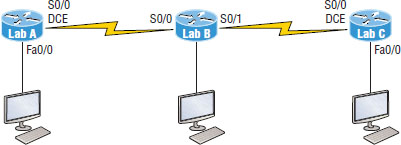
\includegraphics{images/c18f007.jpg}
\caption{}
\end{figure}

\protect\hypertarget{c18.xhtmlux5cux23Page_773}{}{}The first lab (Lab
18.1) requires you to configure three routers for OSPF and then view the
configuration. Note that the labs in this chapter were written to be
used with real equipment---but they can be used with any router
simulator. You can replace the WAN links with Ethernet links if you want
to.

The labs in this chapter are as follows:

\begin{enumerate}
\tightlist
\item
  Lab 18.1: Enabling the OSPF Process
\item
  Lab 18.2: Configuring OSPF Interfaces
\item
  Lab 18.3: Verifying OSPF Operation
\end{enumerate}

\protect\hyperlink{c18.xhtmlux5cux23table18-3}{Table 18.3} shows our IP
addresses for each router (each interface uses a /24 mask).

{\protect\hyperlink{c18.xhtmlux5cux23tableanchor18-3}{\textbf{TABLE~18.3}}
Our IP addresses}

\begin{longtable}[]{@{}lll@{}}
\toprule
Router & Interface & IP address\tabularnewline
\midrule
\endhead
Lab\_A & Fa0/0 & 172.16.10.1\tabularnewline
Lab\_A & S0/0 & 172.16.20.1\tabularnewline
Lab\_B & S0/0 & 172.16.20.2\tabularnewline
Lab\_B & S0/1 & 172.16.30.1\tabularnewline
Lab\_C & S0/0 & 172.16.30.2\tabularnewline
Lab\_C & Fa0/0 & 172.16.40.1\tabularnewline
\bottomrule
\end{longtable}

\subsubsection[Hands-on Lab 18.1: Enabling the OSPF
Process]{\texorpdfstring{\protect\hypertarget{c18.xhtmlux5cux23c18-sec-21}{}{}Hands-on
Lab 18.1: Enabling the OSPF
Process}{Hands-on Lab 18.1: Enabling the OSPF Process}}

This is the first mandatory step in OSPF configuration.

\begin{enumerate}
\item
  Enable OSPF process 100 on Lab\_A:

\begin{verbatim}
Lab_A#conf t
Enter configuration commands, one per line.
  End with CNTL/Z.
Lab_A (config)#router ospf 100
Lab_A (config-router)#^Z
\end{verbatim}
\item
  Enable OSPF process 101 on Lab\_B:

\begin{verbatim}
Lab_B#conf t
Enter configuration commands, one per line.
  End with CNTL/Z.
Lab_B (config)#router ospf 101
Lab_B (config-router)#^Z
\end{verbatim}
\item
  Enable OSPF process 102 on Lab\_C:

\begin{verbatim}
Lab_C#conf t
Enter configuration commands, one per line.
  End with CNTL/Z.
Lab_C (config)#router ospf 102
Lab_C (config-router)#^Z
\end{verbatim}
\end{enumerate}

\subsubsection[Hands-on Lab 18.2: Configuring OSPF
Interfaces]{\texorpdfstring{\protect\hypertarget{c18.xhtmlux5cux23c18-sec-22}{}{}Hands-on
Lab 18.2: Configuring OSPF
Interfaces}{Hands-on Lab 18.2: Configuring OSPF Interfaces}}

The second mandatory step in OSPF is adding your network statements.

\begin{enumerate}
\item
  Configure the LAN and the network between Lab\_A and Lab\_B. Assign it
  to area 0.

\begin{verbatim}
Lab_A#conf t
Enter configuration commands, one per line.
  End with CNTL/Z.
Lab_A (config)#router ospf 100
Lab_A (config-router)#network 172.16.10.1 0.0.0.0 area 0
Lab_A (config-router)#network 172.16.20.1 0.0.0.0 area 0
Lab_A (config-router)#^Z
Lab_A #
\end{verbatim}
\item
  Configure the networks on the Lab\_B router. Assign them to area 0.

\begin{verbatim}
Lab_B#conf t
Enter configuration commands, one per line.
  End with CNTL/Z.
Lab_B(config)#router ospf 101
Lab_B(config-router)#network 172.16.20.2 0.0.0.0 area 0
Lab_B(config-router)#network 172.16.30.1 0.0.0.0 area 0
Lab_B(config-router)#^Z
Lab_B #
\end{verbatim}
\item
  Configure the networks on the Lab\_C router. Assign them to area 0.

\begin{verbatim}
Lab_C#conf t
Enter configuration commands, one per line.
  End with CNTL/Z.
Lab_C(config)#router ospf 102
Lab_C(config-router)#network 172.16.30.2 0.0.0.0 area 0
Lab_C(config-router)#network 172.16.40.1 0.0.0.0 area 0
Lab_C(config-router)#^Z
Lab_C#
\end{verbatim}
\end{enumerate}

\subsubsection[Hands-on Lab 18.3: Verifying OSPF
Operation]{\texorpdfstring{\protect\hypertarget{c18.xhtmlux5cux23c18-sec-23}{}{}Hands-on
Lab 18.3: Verifying OSPF
Operation}{Hands-on Lab 18.3: Verifying OSPF Operation}}

You need to be able to verify what you configure.

\begin{enumerate}
\item
  Execute a \texttt{show\ ip\ ospf\ neighbors} command from the Lab\_A
  router and view the results.

\begin{verbatim}
Lab_A#sho ip ospf neighbors
\end{verbatim}
\item
  Execute a \texttt{show\ ip\ route} command to verify that all other
  routers are learning all routes.

\begin{verbatim}
Lab_A#sho ip route
\end{verbatim}
\item
  Execute a \texttt{show\ ip\ protocols} command to verify OSPF
  information.

\begin{verbatim}
Lab_A#sho ip protocols
\end{verbatim}
\item
  Execute a \texttt{show\ ip\ OSPF} command to verify your RID.

\begin{verbatim}
Lab_A#sho ip ospf
\end{verbatim}
\item
  Execute a \texttt{show\ ip\ ospf\ interface\ f0/0} command to verify
  your timers.

\begin{verbatim}
Lab_A#sho ip ospf int f0/0
\end{verbatim}
\end{enumerate}



\section{Review questions}

\begin{center}\rule{0.5\linewidth}{0.5pt}\end{center}

%\includegraphics{images/note.png}
The following questions are designed to
test your understanding of this chapter's material. For more information
on how to get additional questions, please see
\href{http://www.lammle.com/ccna}{www.lammle.com/ccna}.

\begin{center}\rule{0.5\linewidth}{0.5pt}\end{center}

You can find the answers to these questions in Appendix B, ``Answers to
Review Questions.''

\begin{enumerate}
\item
  There are three possible routes for a router to reach a destination
  network. The first route is from OSPF with a metric of 782. The second
  route is from RIPv2 with a metric of 4. The third is from EIGRP with a
  composite metric of 20514560. Which route will be installed by the
  router in its routing table?

  \begin{enumerate}
  \def\labelenumii{\Alph{enumii}.}
  \tightlist
  \item
    RIPv2
  \item
    EIGRP
  \item
    OSPF
  \item
    All three
  \end{enumerate}
\item
  In the accompanying diagram, which of the routers must be ABRs?
  (Choose all that apply.)

  \begin{figure}
  \centering
  %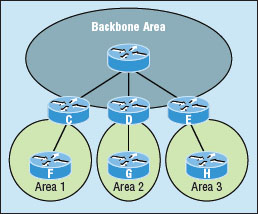
\includegraphics{images/c18f008.jpg}
  \caption{}
  \end{figure}

  \begin{enumerate}
  \def\labelenumii{\Alph{enumii}.}
  \tightlist
  \item
    C
  \item
    D
  \item
    E
  \item
    F
  \item
    G
  \item
    H
  \end{enumerate}
\item
  \protect\hypertarget{c18.xhtmlux5cux23Page_777}{}{}Which of the
  following describe the process identifier that is used to run OSPF on
  a router? (Choose two.)

  \begin{enumerate}
  \def\labelenumii{\Alph{enumii}.}
  \tightlist
  \item
    It is locally significant.
  \item
    It is globally significant.
  \item
    It is needed to identify a unique instance of an OSPF database.
  \item
    It is an optional parameter required only if multiple OSPF processes
    are running on the router.
  \item
    All routes in the same OSPF area must have the same process ID if
    they are to exchange routing information.
  \end{enumerate}
\item
  All of the following must match for two OSPF routers to become
  neighbors except which?

  \begin{enumerate}
  \def\labelenumii{\Alph{enumii}.}
  \tightlist
  \item
    Area ID
  \item
    Router ID
  \item
    Stub area flag
  \item
    Authentication password if using one
  \end{enumerate}
\item
  In the diagram, by default what will be the router ID of Lab\_B?

  \begin{figure}
  \centering
  %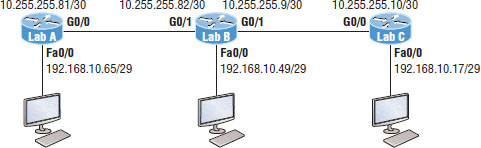
\includegraphics{images/c18f009.jpg}
  \caption{}
  \end{figure}

  \begin{enumerate}
  \def\labelenumii{\Alph{enumii}.}
  \tightlist
  \item
    10.255.255.82
  \item
    10.255.255.9
  \item
    192.168.10.49
  \item
    10.255.255.81
  \end{enumerate}
\item
  You get a call from a network administrator who tells you that he
  typed the following into his router:

\begin{verbatim}
Router(config)#router ospf 1
Router(config-router)#network 10.0.0.0 255.0.0.0 area 0
\end{verbatim}

  He tells you he still can't see any routes in the routing table. What
  configuration error did the administrator make?

  \begin{enumerate}
  \def\labelenumii{\Alph{enumii}.}
  \tightlist
  \item
    The wildcard mask is incorrect.
  \item
    The OSPF area is wrong.
  \item
    \protect\hypertarget{c18.xhtmlux5cux23Page_778}{}{}The OSPF process
    ID is incorrect.
  \item
    The AS configuration is wrong.
  \end{enumerate}
\item
  Which of the following statements is true with regard to the output
  shown?

\begin{verbatim}
Corp#sh ip ospf neighbor
Neighbor ID     Pri   State      Dead Time   Address         Interface
172.31.1.4        1   FULL/BDR   00:00:34    10.10.10.2     FastEthernet0/0
192.168.20.1      0   FULL/  -   00:00:31    172.16.10.6     Serial0/1
192.168.10.1      0   FULL/  -   00:00:32    172.16.10.2     Serial0/0
\end{verbatim}

  \begin{enumerate}
  \def\labelenumii{\Alph{enumii}.}
  \tightlist
  \item
    There is no DR on the link to 192.168.20.1.
  \item
    The Corp router is the BDR on the link to 172.31.1.4.
  \item
    The Corp router is the DR on the link to 192.168.20.1.
  \item
    The link to 192.168.10.1 is Active.
  \end{enumerate}
\item
  What is the administrative distance of OSPF?

  \begin{enumerate}
  \def\labelenumii{\Alph{enumii}.}
  \tightlist
  \item
    90
  \item
    100
  \item
    120
  \item
    110
  \end{enumerate}
\item
  In OSPF, Hellos are sent to what IP address?

  \begin{enumerate}
  \def\labelenumii{\Alph{enumii}.}
  \tightlist
  \item
    224.0.0.5
  \item
    224.0.0.9
  \item
    224.0.0.10
  \item
    224.0.0.1
  \end{enumerate}
\item
  What command generated the following output?

\begin{verbatim}
172.31.1.4        1   FULL/BDR   00:00:34    10.10.10.2     FastEthernet0/0
192.168.20.1      0   FULL/  -   00:00:31    172.16.10.6     Serial0/1
192.168.10.1      0   FULL/  -   00:00:32    172.16.10.2     Serial0/0
\end{verbatim}

  \begin{enumerate}
  \def\labelenumii{\Alph{enumii}.}
  \tightlist
  \item
    \texttt{show\ ip\ ospf\ neighbor}
  \item
    \texttt{show\ ip\ ospf\ database}
  \item
    \texttt{show\ ip\ route}
  \item
    \texttt{show\ ip\ ospf\ interface}
  \end{enumerate}
\item
  Updates addressed to 224.0.0.6 are destined for which type of OSPF
  router?

  \begin{enumerate}
  \def\labelenumii{\Alph{enumii}.}
  \tightlist
  \item
    DR
  \item
    ASBR
  \item
    \protect\hypertarget{c18.xhtmlux5cux23Page_779}{}{}ABR
  \item
    All OSPF routers
  \end{enumerate}
\item
  For some reason, you cannot establish an adjacency relationship on a
  common Ethernet link between two routers. Looking at this output, what
  is the cause of the problem?

\begin{verbatim}
RouterA#
Ethernet0/0 is up, line protocol is up
  Internet Address 172.16.1.2/16, Area 0
  Process ID 2, Router ID 172.126.1.2, Network Type BROADCAST, Cost: 10
  Transmit Delay is 1 sec, State DR, Priority 1
  Designated Router (ID) 172.16.1.2, interface address 172.16.1.1
  No backup designated router on this network
  Timer intervals configured, Hello 5, Dead 20, Wait 20, Retransmit 5
 
RouterB#
Ethernet0/0 is up, line protocol is up
  Internet Address 172.16.1.1/16, Area 0
  Process ID 2, Router ID 172.126.1.1, Network Type BROADCAST, Cost: 10
  Transmit Delay is 1 sec, State DR, Priority 1
  Designated Router (ID) 172.16.1.1, interface address 172.16.1.2
  No backup designated router on this network
  Timer intervals configured, Hello 10, Dead 40, Wait 40, Retransmit 5
\end{verbatim}

  \begin{enumerate}
  \def\labelenumii{\Alph{enumii}.}
  \tightlist
  \item
    The OSPF area is not configured properly.
  \item
    The priority on RouterA should be set higher.
  \item
    The cost on RouterA should be set higher.
  \item
    The Hello and Dead timers are not configured properly.
  \item
    A backup designated router needs to be added to the network.
  \item
    The OSPF process ID numbers must match.
  \end{enumerate}
\item
  In the work area, match each OSPF term (by line) to its definition.

  \begin{figure}
  \centering
  %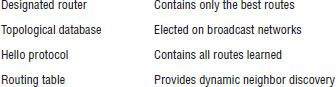
\includegraphics{images/c18f010.jpg}
  \caption{}
  \end{figure}
\item
  Type the command that will disable OSPF on the Fa0/1 interface under
  the routing process. Write only the command and not the prompt.
\item
  \protect\hypertarget{c18.xhtmlux5cux23Page_780}{}{}Which two of the
  following commands will place network 10.2.3.0/24 into area 0? (Choose
  two.)

  \begin{enumerate}
  \def\labelenumii{\Alph{enumii}.}
  \tightlist
  \item
    \texttt{router\ eigrp\ 10}
  \item
    \texttt{router\ ospf\ 10}
  \item
    \texttt{router\ rip}
  \item
    \texttt{network\ 10.0.0.0}
  \item
    \texttt{network\ 10.2.3.0\ 255.255.255.0\ area\ 0}
  \item
    \texttt{network\ 10.2.3.0\ 0.0.0.255\ area0}
  \item
    \texttt{network\ 10.2.3.0\ 0.0.0.255\ area\ 0}
  \end{enumerate}
\item
  Given the following output, which statement or statements can be
  determined to be true? (Choose all that apply.)

\begin{verbatim}
RouterA2# show ip ospf neighbor
 
Neighbor ID Pri State Dead Time Address Interface
192.168.23.2 1 FULL/BDR 00:00:29 10.24.4.2 FastEthernet1/0
192.168.45.2 2 FULL/BDR 00:00:24 10.1.0.5 FastEthernet0/0
192.168.85.1 1 FULL/- 00:00:33 10.6.4.10 Serial0/1
192.168.90.3 1 FULL/DR 00:00:32 10.5.5.2 FastEthernet0/1
192.168.67.3 1 FULL/DR 00:00:20 10.4.9.20 FastEthernet0/2
192.168.90.1 1 FULL/BDR 00:00:23 10.5.5.4 FastEthernet0/1
<<output omitted>>
\end{verbatim}

  \begin{enumerate}
  \def\labelenumii{\Alph{enumii}.}
  \tightlist
  \item
    The DR for the network connected to Fa0/0 has an interface priority
    higher than 2.
  \item
    This router (A2) is the BDR for subnet 10.1.0.0.
  \item
    The DR for the network connected to Fa0/1 has a router ID of
    10.5.5.2.
  \item
    The DR for the serial subnet is 192.168.85.1.
  \end{enumerate}
\item
  What are three reasons for creating OSPF in a hierarchical design?
  (Choose three.)

  \begin{enumerate}
  \def\labelenumii{\Alph{enumii}.}
  \tightlist
  \item
    To decrease routing overhead
  \item
    To speed up convergence
  \item
    To confine network instability to single areas of the network
  \item
    To make configuring OSPF easier
  \end{enumerate}
\item
  Type the command that produced the following output. Write only the
  command and not the prompt.

\begin{verbatim}
FastEthernet0/0 is up, line protocol is up
  Internet Address 10.10.10.1/24, Area 0
  Process ID 1, Router ID 223.255.255.254, Network Type BROADCAST, Cost: 
1 Transmit Delay is 1 sec, State DR, Priority 1
  Designated Router (ID) 223.255.255.254, Interface address 10.10.10.1
Backup Designated router (ID) 172.31.1.4, Interface address 10.10.10.2
Timer intervals configured, Hello 10, Dead 40, Wait 40, Retransmit 5
    oob-resync timeout 40
    Hello due in 00:00:08
  Supports Link-local Signaling (LLS)
  Cisco NSF helper support enabled
  IETF NSF helper support enabled
  Index 3/3, flood queue length 0
  Next 0x0(0)/0x0(0)
  Last flood scan length is 1, maximum is 1
  Last flood scan time is 0 msec, maximum is 0 msec
  Neighbor Count is 1, Adjacent neighbor count is 1
    Adjacent with neighbor 172.31.1.  Suppress hello for 0 neighbor(s)
\end{verbatim}
\item
  A(n) \_\_\_\_\_\_\_\_\_\_ is an OSPF data packet containing link-state
  and routing information that is shared among OSPF routers.

  \begin{enumerate}
  \def\labelenumii{\Alph{enumii}.}
  \tightlist
  \item
    LSA
  \item
    TSA
  \item
    Hello
  \item
    SPF
  \end{enumerate}
\item
  If routers in a single area are configured with the same priority
  value, what value does a router use for the OSPF router ID in the
  absence of a loopback interface?

  \begin{enumerate}
  \def\labelenumii{\Alph{enumii}.}
  \tightlist
  \item
    The lowest IP address of any physical interface
  \item
    The highest IP address of any physical interface
  \item
    The lowest IP address of any logical interface
  \item
    The highest IP address of any logical interface
  \end{enumerate}
\end{enumerate}
